\section{Design of \textsf{PCStream}}
In this section, we describe in detail the proposed automatic stream management technique, %shane part
\textsf{\small PCStream}.  We first explain how we automatically extract PCs during
runtime and describe how multiple PCs are mapped to streams in an SSD.
In order to mitigate the side effect of a few outlier PCs with large lifetime variances, 
we introduce `substreams' based on a two-phase
stream assignment technique.
%{\it The PC extractor module}, which is implemented in the ... as part ... of a
%system call handler, computes a PC signature (i.e., a sum of program counter
%values) for each write-related system function. 추가 동작 설명..


Fig.~\ref{fig:architecture} shows an overall organization of \textsf{\small PCStream}.
\textit{The PC extractor module}, which is implemented in the Linux kernel as
part of a system call handler, 
computes a PC signature, which is used as a unique ID for each program context.  
We use the signature program counter~\cite{PC} as a PC signature 
by summing program counter values along the execution path to a write-related system function 
(e.g., {\tt write()}).  
With the PC signature, we can monitor the data lifetime of each write at the program context level. 
A PC signature value is stored
in an inode data structure of a file system (modified for \textsf{\small PCStream})
and is delivered to \textit{the lifetime analyzer module} which estimates
expected lifetimes of data belonging to a given PC in the block device level.
In order to efficiently detect the end of data lifetime in append-only
workloads, the lifetime analyzer also intercepts TRIM~\cite{TRIM} requests from a file system.  %shane part
Based on the lifetime information, \textit{the PC-to-stream
mapper module} clusters PCs with similar lifetimes and maps them together to
the same stream ID.  This mapping is required because 
the number of streams in an SSD is generally less than the number of PCs in host applications.

\subsection{External Stream Management}
\subsubsection{Automatic PC computation}
As mentioned earlier, a PC is represented by a PC signature which is defined as
the sum of program counter values along the execution path of a function call that
finally reaches a write-related system function. A function call involves
pushing the next program counter, which is used as a return address, to the
stack followed by pushing a frame pointer value.  In general, by using frame
pointer values, we are able to back-track the stack frames of the process and
selectively get return addresses for generating a PC signature.  For example,
Fig.~\ref{fig:getpc}(a) shows the abstracted execution path for flushing data
in RocksDB and Fig.~\ref{fig:getpc}(b) illustrates how a PC signature is obtained
by back-tracking the stack.  
Since a frame pointer value in the stack holds the address of the previous
frame pointer, the PC extractor can easily obtain return addresses and
accumulate them to compute a PC signature. 
(The return addresses are pushed
before calling the \textsf{\small  write()}, \textsf{\small  BuildTable()} and \textsf{\small 
WriteLevel0Table()} functions.)

\begin{figure}[t]
	\centering
	%\vspace{-10pt}
	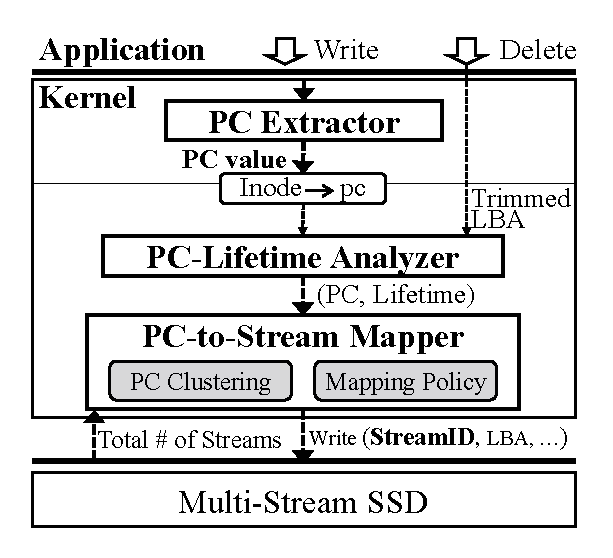
\includegraphics[width=0.6\linewidth]{figure/architecture4}
	%\vspace{-9pt}
	\caption{An overall architecture of \textsf{\small PCStream}.}
	\label{fig:architecture}
	%\vspace{-22pt}
\end{figure}


The frame pointer-based approach for computing PC signatures, however, is not
always possible because modern C/C++ compilers often do not use the frame
pointer for improving the efficiency of register allocation.
One example is a
{\tt -fomit-frame-pointer} option of GCC~\cite{GCC}. 
Although this option allows the frame pointer to be used as a general-purpose
register for high performance, it makes very difficult for us to back-track
return addresses along the call chains.  

\begin{figure}[b]
%	\vspace{-10pt}
	\centering
	%\vspace{-8pt}
	\subfloat[An abstracted execution path for flushing data.]{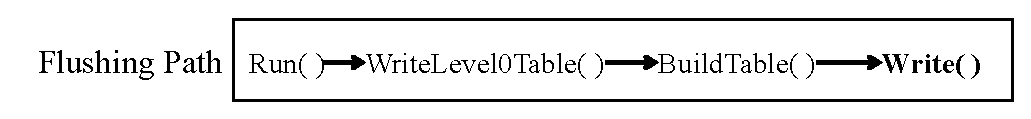
\includegraphics[width=0.4\textwidth]{figure/getpc_1}}  
	%\vspace{-14pt}
	\hfill
	\subfloat[with the frame pointer.]{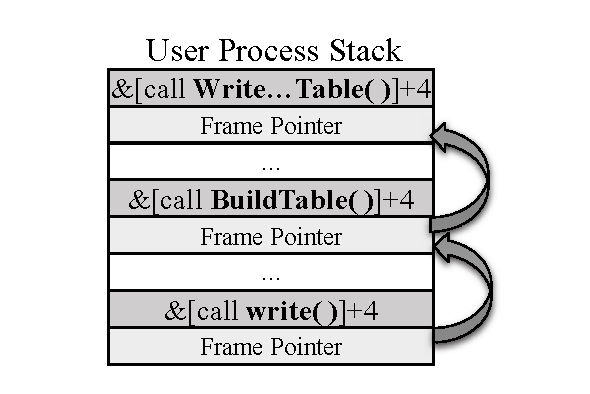
\includegraphics[width=0.22\textwidth]{figure/getpc_2}}
	\subfloat[without the frame pointer.]{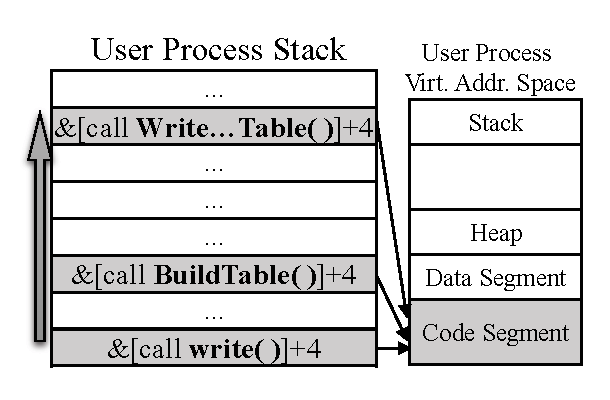
\includegraphics[width=0.22\textwidth]{figure/getpc_3}}
	%\vspace{-9pt}
	%\caption{An example execution path and its PC extraction methods.}
	\caption{An example execution path and its PC extraction.} %shane part
	\label{fig:getpc}
	%\vspace{-20pt}
\end{figure}

In \textsf{\small PCStream}, we employ a simple but effective workaround 
for backtracking the call stack when the frame pointer is not used.
When a write system call is made, we scan every word in the stack and check
if it belongs to the process's code segment.  If the scanned stack word holds a
value within the address range of the code segment, we assume that it is a
return address.  Since scanning the full stack takes too long, we stop the
stack scanning procedure when a sufficient number of return address candidates
are found.  In the current version, we stop when 5 return address candidates
are found.  Although quite ad-hoc, a restricted scan is effective in
distinguishing different PCs because two different PCs
cannot follow the same execution path to write system functions.  
(If they do, they are the same PC.) In our evaluation
with a 3.4 GHz CPU machine, the performance overhead of the restricted scan was
almost negligible, taking only 300-400 $n$sec per write system call.

\subsubsection{Computing PC for Indirect Writes}
+ JVM (cassandra), mmap (mongo DB), internal buffer (mysql) - future work \\ \\

\subsubsection{PC lifetime management}
+ maintaining PC information for repeated executing application (hashing) \\ \\
The prediction of PC lifetimes is rather complicated. 
The data lifetime of the append-only workload is defined 
from when a write request is issued until the TRIM command~\cite{TRIM} is issued to 
the corresponding address.
In order to measure the lifetime of data, the lifetime analyzer 
records the write time and PC value for each write request using its LBA.
Upon receiving the TRIM command, the lifetime analyzer can compute the 
lifetime of the corresponding data using the recorded information.
Note that, the
same PC may generate multiple data streams with different lifetimes.
We take the average lifetime as the PC's lifetime.

\subsubsection{Mapping PCs to SSD streams}

The last step in \textsf{\small PCStream} is to map
a group of PCs with similar lifetimes to an SSD stream.
This is because each SSD supports a limited number of stream IDs. For
example, SSDs used in \textsf{\small FStream}~\cite{FStream} and \textsf{\small AutoStream}~\cite{AutoStream}
support only 9 and 16 streams, respectively. To properly group multiple PCs,
the PC-to-stream mapper employs a simple 1-D clustering algorithm. 
In order to cluster PCs with similar lifetimes, the mapper calculates the 
lifetime difference between PCs.
Then, PCs with the smallest lifetime difference are clustered into the same PC group. 
The mapper repeats this clustering step until all the PCs are assigned to their PC groups.
For adapting to changing
workloads, reclustering operations should be regularly performed. Since the
number of PCs created by applications is not limited, the clustering algorithm
must be efficient enough to quickly handle many PCs. Our goal in this work is
to confirm the feasibility of using PCs, so we leave
those issues as our future work.

\subsection{Internal Stream Management}
\subsubsection{Low resource requirement of IOS}

In Section 2.2.1, we describe various resource overheads that limit the number of external streams.
In the case of an internal stream used for internal data migration of SSD, 
it has a relatively small resource overhead due to its distinguishing characteristics from the external stream.

Unlike external streams, which are handled directly by host requests,
since the internal stream can be processed as a background operation, 
performance degradation may not occur even if the data structure is located in a relatively slow memory.
However, the saturation condition, which requires GC to be continuously executed during write processing, 
may cause performance degradation due to relatively slow memory usage.

With regard to power resources, buffering can be used for flash parallelism even during data migration, but there is a big difference in that no power resource is required to guarantee data integrity.
In the case of buffering data for host write, if data is not stored in flash when power off, data is lost. 
However, in the case of buffering data during data migration, since the original data always exists in the source block of migration, there is no problem in ensuring data integrity without special handling or power resource requirement.

The increase of the active point for data migration has the problem that WAF might be increased by reducing the overprovision area. 
However, in most workloads, the benefit of using WAF reduction with multiple internal streams in data migration has the advantage of offsetting the increase in WAF due to overprovision area reduction and lowering the overall WAF.


\subsubsection{IOS Management}
+ explain block utilization trade-off, deciding number of IOS and mapping \\ \\ 

